\documentclass[landscape]{sciposter}

\usepackage{amsmath}
\usepackage{graphicx}
\usepackage{IEEEtrantools}
\usepackage{multicol}
\usepackage{setspace}
\usepackage{algorithmic}

\onehalfspacing
%\multicoltolerance = 1000
%\raggedcolumns

\title{Metropolis-Hastings Implementations of the Forward-Filtering-Backward-Sampling \\ Algorithm for Particle Smoothing}

\author{P. Bunch and S. Godsill}
\institute{Department of Engineering, University of Cambridge, Trumpington Street, Cambridge, CB2 1PZ, UK}
\email{\{pb404,sjg\}@eng.cam.ac.uk}

\leftlogo[2]{CUnibig.pdf}

\renewcommand{\titlesize}{\huge}

\begin{document}

\maketitle
\begin{multicols}{4}

\begin{abstract}
The conventional forward-filtering-backward-sampling algorithm for particle smoothing generates samples from the joint smoothing distribution by sequentially sampling backwards from the forward filter approximations. This algorithm has a computational complexity quadratic in the number of particles, which is often restrictive. In addition, the support of the smoothing distribution is restricted to the values which appear in the filtering approximation. Here a Metropolis-Hastings sampling procedure is used to improve the efficiency of the forward-filtering-backward-sampling algorithm, achieving comparable error performance but with a lower execution time. In addition, an algorithm for approximating the joint smoothing distribution without limited support is presented, which achieves simultaneous improvements in both execution time and error. These algorithms also provide a greater degree of flexibility over existing methods, allowing a trade-off between execution time and estimation error, controlled by the length of the Markov chains.
\end{abstract}

%\columnbreak

\section*{Introduction}

Consider a standard hidden Markov model for Bayesian inference,
%
\begin{IEEEeqnarray*}{rCl}
x_{k} & \sim & p(x_{k}|x_{k-1}) \\
y_{k} & \sim & p(y_{k}|x_{k})      .
\end{IEEEeqnarray*}

We address the task of joint smoothing --- inference of $p(x_{1:K}|y_{1:K})$ (where $K$ is the number of time steps).

%Commonly of interest are the problems of filtering and smoothing. Filtering is the inference of $p(x_k|y_{1:k})$. There are two related smoothing tasks:
%\begin{itemize}
%  \item Joint smoothing --- inference of $p(x_{1:K}|y_{1:K})$ (where $K$ is the number of time steps).
%  \item Marginal smoothing --- inference of $p(x_{k}|y_{1:K})$ for each $k$.
%\end{itemize}
%Here we are concerned with joint smoothing.

For non-linear, non-Gaussian models, numerical approximations are needed. Particle methods represent posterior distributions with a set of samples \cite{Doucet2009}.
\begin{itemize}
  \item Filter: $\hat{p}(x_{k}|y_{1:k}) = \sum_i w_k^{(i)} \delta_{x_k^{(i)}}(x_k)$.
  \item Smoother: $\hat{p}(x_{1:K}|y_{1:K}) = \sum_i w_K^{(i)} \delta_{x_{1:K}^{(i)}}(x_{1:K})$.
\end{itemize}



\section*{Forward-Filtering-Backward-Sampling}

The forward-filtering-backward-sampling (FFBS) algorithm \cite{Godsill2004} draws particles from the joint smoothing distribution by sequentially sampling a set of backwards conditional distributions,
%
\begin{IEEEeqnarray*}{rCl}
p(x_{1:K}|y_{1:K}) & = & p(x_K|y_{1:K}) \prod_{k=1}^{K-1} p(x_k|x_{k+1}, y_{1:K})     .
\end{IEEEeqnarray*}

The conditional factors may be expressed as,
%
\begin{IEEEeqnarray*}{rCl}
p(x_k|\tilde{x}_{k+1}, y_{1:K}) & =       & p(x_k|\tilde{x}_{k+1}, y_{1:k})   \\
                                & \propto & p(\tilde{x}_{k+1}|x_k) p(x_k|y_{1:k})   .
\end{IEEEeqnarray*}

where $\tilde{x}_{k+1}$ is the future state already sampled. Using the filter approximations, the backwards conditional distributions are approximated as,
%
\begin{IEEEeqnarray*}{rCl}
\hat{p}(x_k|\tilde{x}_{k+1}, y_{1:K}) & = & \sum_i  \tilde{w}_k^{(i)} \delta_{x_{k}^{(i)}}(x_{k})    \\
\tilde{w}_k^{(i)} & \propto & w_k^{(i)} p(\tilde{x}_{k+1}|x_k^{(i)})      .
\end{IEEEeqnarray*}

This may be sampled easily by calculating $\tilde{w}_k^{(i)}$ for each of the $N_F$ filter particles and sampling the resulting multinomial distribution. The whole procedure is repeated $N_S$ times, once for each smoothing particle.

\begin{algorithm}
\begin{algorithmic}[1]
\linespread{1.7} \selectfont
 	\STATE Run a particle filter to approximate $p(x_k|y_{1:k})$ for each $k$ and store the resulting particles $\{x_k^{(i)}, w_k^{(i)}\}$.
	\FOR{$i = 1$ \TO $N_S$}
		\STATE Sample $\tilde{x}_{K}^{(i)} \sim \hat{p}(x_K|y_{1:K})$.
		\FOR{$k = K-1$ \TO $1$}
            \STATE Sample $\tilde{x}_{k}^{(i)} \sim p(x_k|\tilde{x}_{k+1}, y_{1:K})$. This is the critical step. See text for various methods.
%			\FOR{$j = 1$ \TO $N_F$}
%				\STATE Calculate weight $\tilde{w}_k^{(j)} = w_k^{(j)} p(\tilde{x}_{k+1}|x_k^{(j)})$.
%			\ENDFOR
%			\STATE Sample $\tilde{x}_{k}^{(i)} \sim \sum_j \tilde{w}_k^{(j)} \delta_{x_{k}^{(j)}}(x_{k})$.
		\ENDFOR
	\ENDFOR
\end{algorithmic}
\caption{Forward-filtering-backward-sampling algorithm}
\end{algorithm}



\subsection*{Deficiencies}
%
The basic FFBS algorithm suffers from two drawbacks:
\begin{itemize}
  \item The algorithmic complexity is $\mathcal{O}(N_F \times N_S)$ which is restrictive.
  \item The support for the smoothing approximation is limited to the values appearing in the filtering particles.
\end{itemize}



\section*{A Metropolis-Hastings implementation}

The FFBS bottleneck is the calculation of the $N_F$ backwards weights for every sampling step, in order to sample from $\hat{p}(x_k|\tilde{x}_{k+1}, y_{1:K})$. Instead, we can sample this distribution using Metropolis-Hastings (MH).

\begin{itemize}
  \item The filter weights are used to propose particles from $\hat{p}(x_k | y_{1:k})$.
  \item The new state, $x_k^*$, replaces the old state, $x_k$ with acceptance probability,
\end{itemize}
%
\begin{IEEEeqnarray*}{rCl}
\alpha &=& \min \Bigg[1, \frac{ p(\tilde{x}_{k+1}|x_k^{*}) }{ p(\tilde{x}_{k+1}|x_k) }  \Bigg]     .
\end{IEEEeqnarray*}



\columnbreak

\subsection*{Initialisation}
%
\begin{itemize}
  \item An initial value is required to start the chain.
  \item Instead of sampling the state, $x_k$, at each step, sample the entire history, $x_{1:k}$.
  \item No additional states need be stored, only index of the $(k-1)$-time particle from which each $k$-time particle originates.
  \item No burn-in required --- initial state is drawn from target distribution.
\end{itemize}



\subsection*{Effects}
%
\begin{itemize}
  \item Computational complexity reduced to $\mathcal{O}(M \times N_S)$, where $M$ is the  length of Markov chains.
  \item $M = 0$ reproduces particles from the filter smoother. $M \rightarrow \infty$ draws an independent sample from the distribution.
  \item Performance expected to be bounded by that of the filter smoother and the standard FFBS.
  \item Much faster than FFBS when $M$ can be made small, i.e. when acceptance rate is high.
\end{itemize}

%\begin{algorithm}
%\begin{algorithmic}[1]
%%\linespread{1.7} \selectfont
% 	\STATE Run a particle filter to approximate $p(x_{1:k}|y_{1:k})$ for each $k$ and store the resulting particles $\{x_{1:k}^{(i)}, w_k^{(i)}\}$.
%	\FOR{$i = 1$ \TO $N_S$}
%		\STATE Sample $\tilde{x}_{1:K}^{(i)} \sim \sum_j w_K^{(j)} \delta_{x_{1:K}^{(j)}}(x_{1:K})$.
%		\FOR{$k = K-1$ \TO $1$}
%			\STATE $x_{1:k}^{(i)(0)} \gets \tilde{x}_{1:k}^{(i)}$.
%			\FOR{$m = 1$ \TO $M$}
%				\STATE Propose a new state, $x_{1:k}^{(i)*} \sim \sum_j \tilde{v}_k^{(j)} \delta_{x_{1:k}^{(j)}}(x_{1:k})$.
%				\STATE With probability $\alpha$,\\ $x_{1:k}^{(i)(m)} \gets x_{1:k}^{(i)*}$. Otherwise, $x_{1:k}^{(i)(m)} \gets x_{1:k}^{(i)(m-1)}$.
%			\ENDFOR
%			\STATE $\tilde{x}_{1:k}^{(i)} \gets x_{1:k}^{(i)(M)}$
%		\ENDFOR
%	\ENDFOR
%\end{algorithmic}
%\caption{Metropolis-Hastings forward-filtering-backward-sampling (MH-FFBS) algorithm}
%\end{algorithm}



\subsection*{Alternatives}
%
Rejection sampling \cite{Douc2011} can achieve a similar complexity reduction.
\begin{itemize}
  \item Rejection sampling can be very slow if rejection rates are high, e.g. when state dimension high.
  \item MH method more flexible --- chain length can be set to trade-off complexity against running time.
\end{itemize}




\section*{Improving the Support}

Modify the MH proposal to use,
%
\begin{IEEEeqnarray*}{c}
\hat{p}(x_{1:k-1}|y_{1:k-1}) q(x_k|x_{k-1}, \tilde{x}_{k+1}, y_k)     .
\end{IEEEeqnarray*}

Support of $x_k$ is no longer restricted to those values appearing in the filter approximation. This is inspired by the method used in \cite{Fearnhead2010} for two-filter marginal smoothing.

Acceptance probability is now,
%
\begin{IEEEeqnarray*}{rCl}
\alpha &=& \min \Bigg[ 1, \frac{  p(\tilde{x}_{k+1}|x_k^{*}) p(x_k^{*}|x_{k-1}^{*}) p(y_k|x_k^{*}) q(x_k|x_{k-1},\tilde{x}_{k+1},y_k) }{ p(\tilde{x}_{k+1}|x_k) p(x_k|x_{k-1}) p(y_k|x_k) q(x_k^{*}|x_{k-1}^{*},\tilde{x}_{k+1},y_k) }  \Bigg]      .
\end{IEEEeqnarray*}

%\begin{algorithm}
%\begin{algorithmic}[1]
%%\linespread{1.7} \selectfont
% 	\STATE Run a particle filter to approximate $p(x_{1:k}|y_{1:k})$ for each $k$.
%	\FOR{$i = 1$ \TO $N_S$}
%		\STATE Sample $\tilde{x}_{1:K}^{(i)} \sim \sum_j w_K^{(j)} \delta_{x_{1:K}^{(j)}}(x_{1:K})$.
%		\FOR{$k = K-1$ \TO $1$}
%			\STATE $x_{1:k}^{(i)(0)} \gets \tilde{x}_{1:k}^{(i)}$.
%			\FOR{$m = 1$ \TO $M$}
%				\STATE Propose a new state history,\\ $x_{1:k-1}^{(i)*} \sim \sum_j \tilde{v}_{k-1}^{(j)} \delta_{x_{1:k-1}^{(j)}}(x_{1:k-1})$.
%				\STATE Propose a new state, $x_{k}^{(i)*} \sim q(x_k|x_{k-1}^{*},\tilde{x}_{k+1},y_k)$.
%				\STATE With probability $\alpha$,\\ $x_{1:k}^{(i)(m)} \gets x_{1:k}^{(i)*}$. Otherwise, $x_{1:k}^{(i)(m)} \gets x_{1:k}^{(i)(m-1)}$.
%			\ENDFOR
%			\STATE $\tilde{x}_{1:k}^{(i)} \gets x_{1:k}^{(i)(M)}$
%		\ENDFOR
%	\ENDFOR
%\end{algorithmic}
%\caption{Metropolis-Hastings forward-filtering-backward-proposing (MH-FFBP) algorithm}
%\end{algorithm}



%\columnbreak

\section*{Demonstrations}

New algorithms tested on a simulated tracking problem with near constant velocity dynamic model and range-bearing observation model. Two observation covariance cases are considered.
%
\begin{figure}
\centering
\subfigure[Case 1]{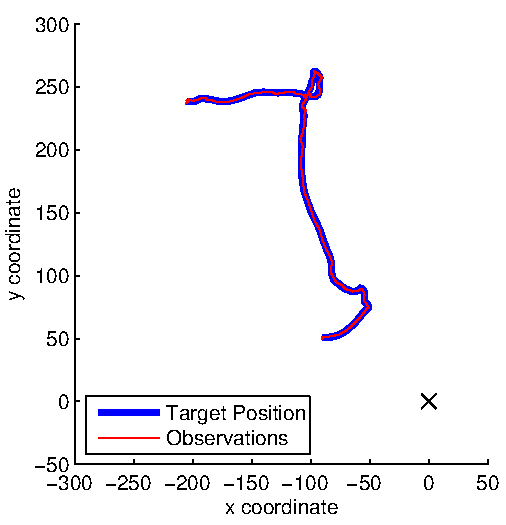
\includegraphics[width=0.45\columnwidth]{POSTER_case1_trajectory.pdf}}
\subfigure[Case 2]{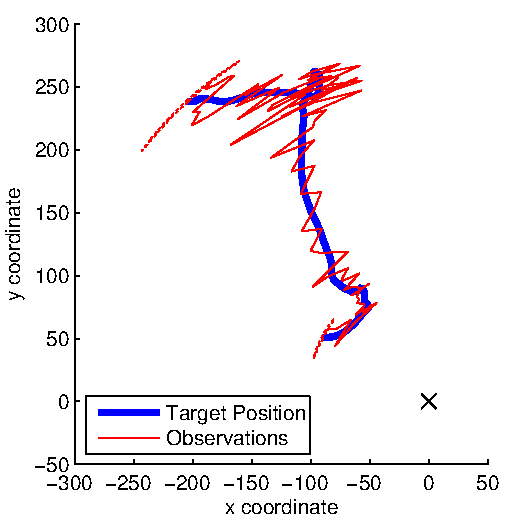
\includegraphics[width=0.45\columnwidth]{POSTER_case2_trajectory.pdf}}
\caption{Example trajectory with observations from the two noise covariance cases. Constant likelihood contours are shown for the first and last position (dashed)}
\end{figure}

\begin{figure}[!t]
\centering
\subfigure[Case 1]{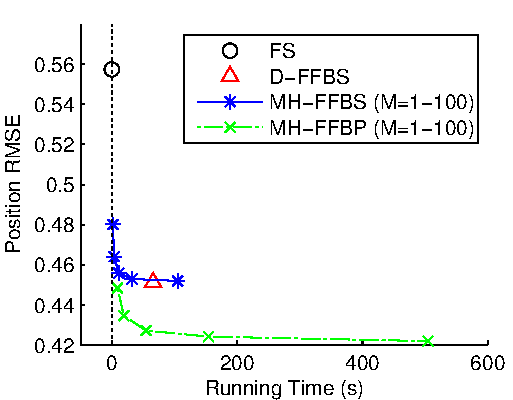
\includegraphics[width=0.45\columnwidth]{POSTER_case1_smoother_comparison_posRMSE_time.pdf}}
\subfigure[Case 2]{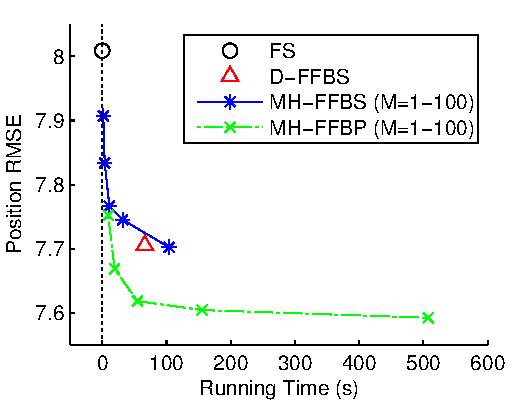
\includegraphics[width=0.45\columnwidth]{POSTER_case2_smoother_comparison_posRMSE_time.pdf}}
\caption{Position RMSEs and running times of various smoothing algorithms with two noise covariance cases.}%
\end{figure}



\section*{Conclusions}

\begin{itemize}
  \item New smoothing algorithms achieve lower error for a given running time. Similar results apply to consistency of estimates.
  \item Chain length provides flexibility to trade-off running time against quality of estimate.
\end{itemize}


{\small
\bibliographystyle{IEEEtran}
\bibliography{D:/pb404/Dropbox/PhD/Cleanbib}
}

\end{multicols}

\end{document}